
% Supõe-se que, na introdução, tenha sido posto a definição do problema de SQA como a necessidade de garantir um sinal de boa qualidade, seja para humanos não cometerem enganos, seja para modelos preditivos serem capazes de estimar com acurácia.

In this chapter I present the literature of the \acrlong{SQA} of cardiological signals problem. To better organize the analysis, I divided it into the sections, as we see in the Figure \ref{fig:SubjectTree}: Problem, Feature Extraction Method, Dimensionality and Projection Method.

\begin{figure}[t]
	\centering
	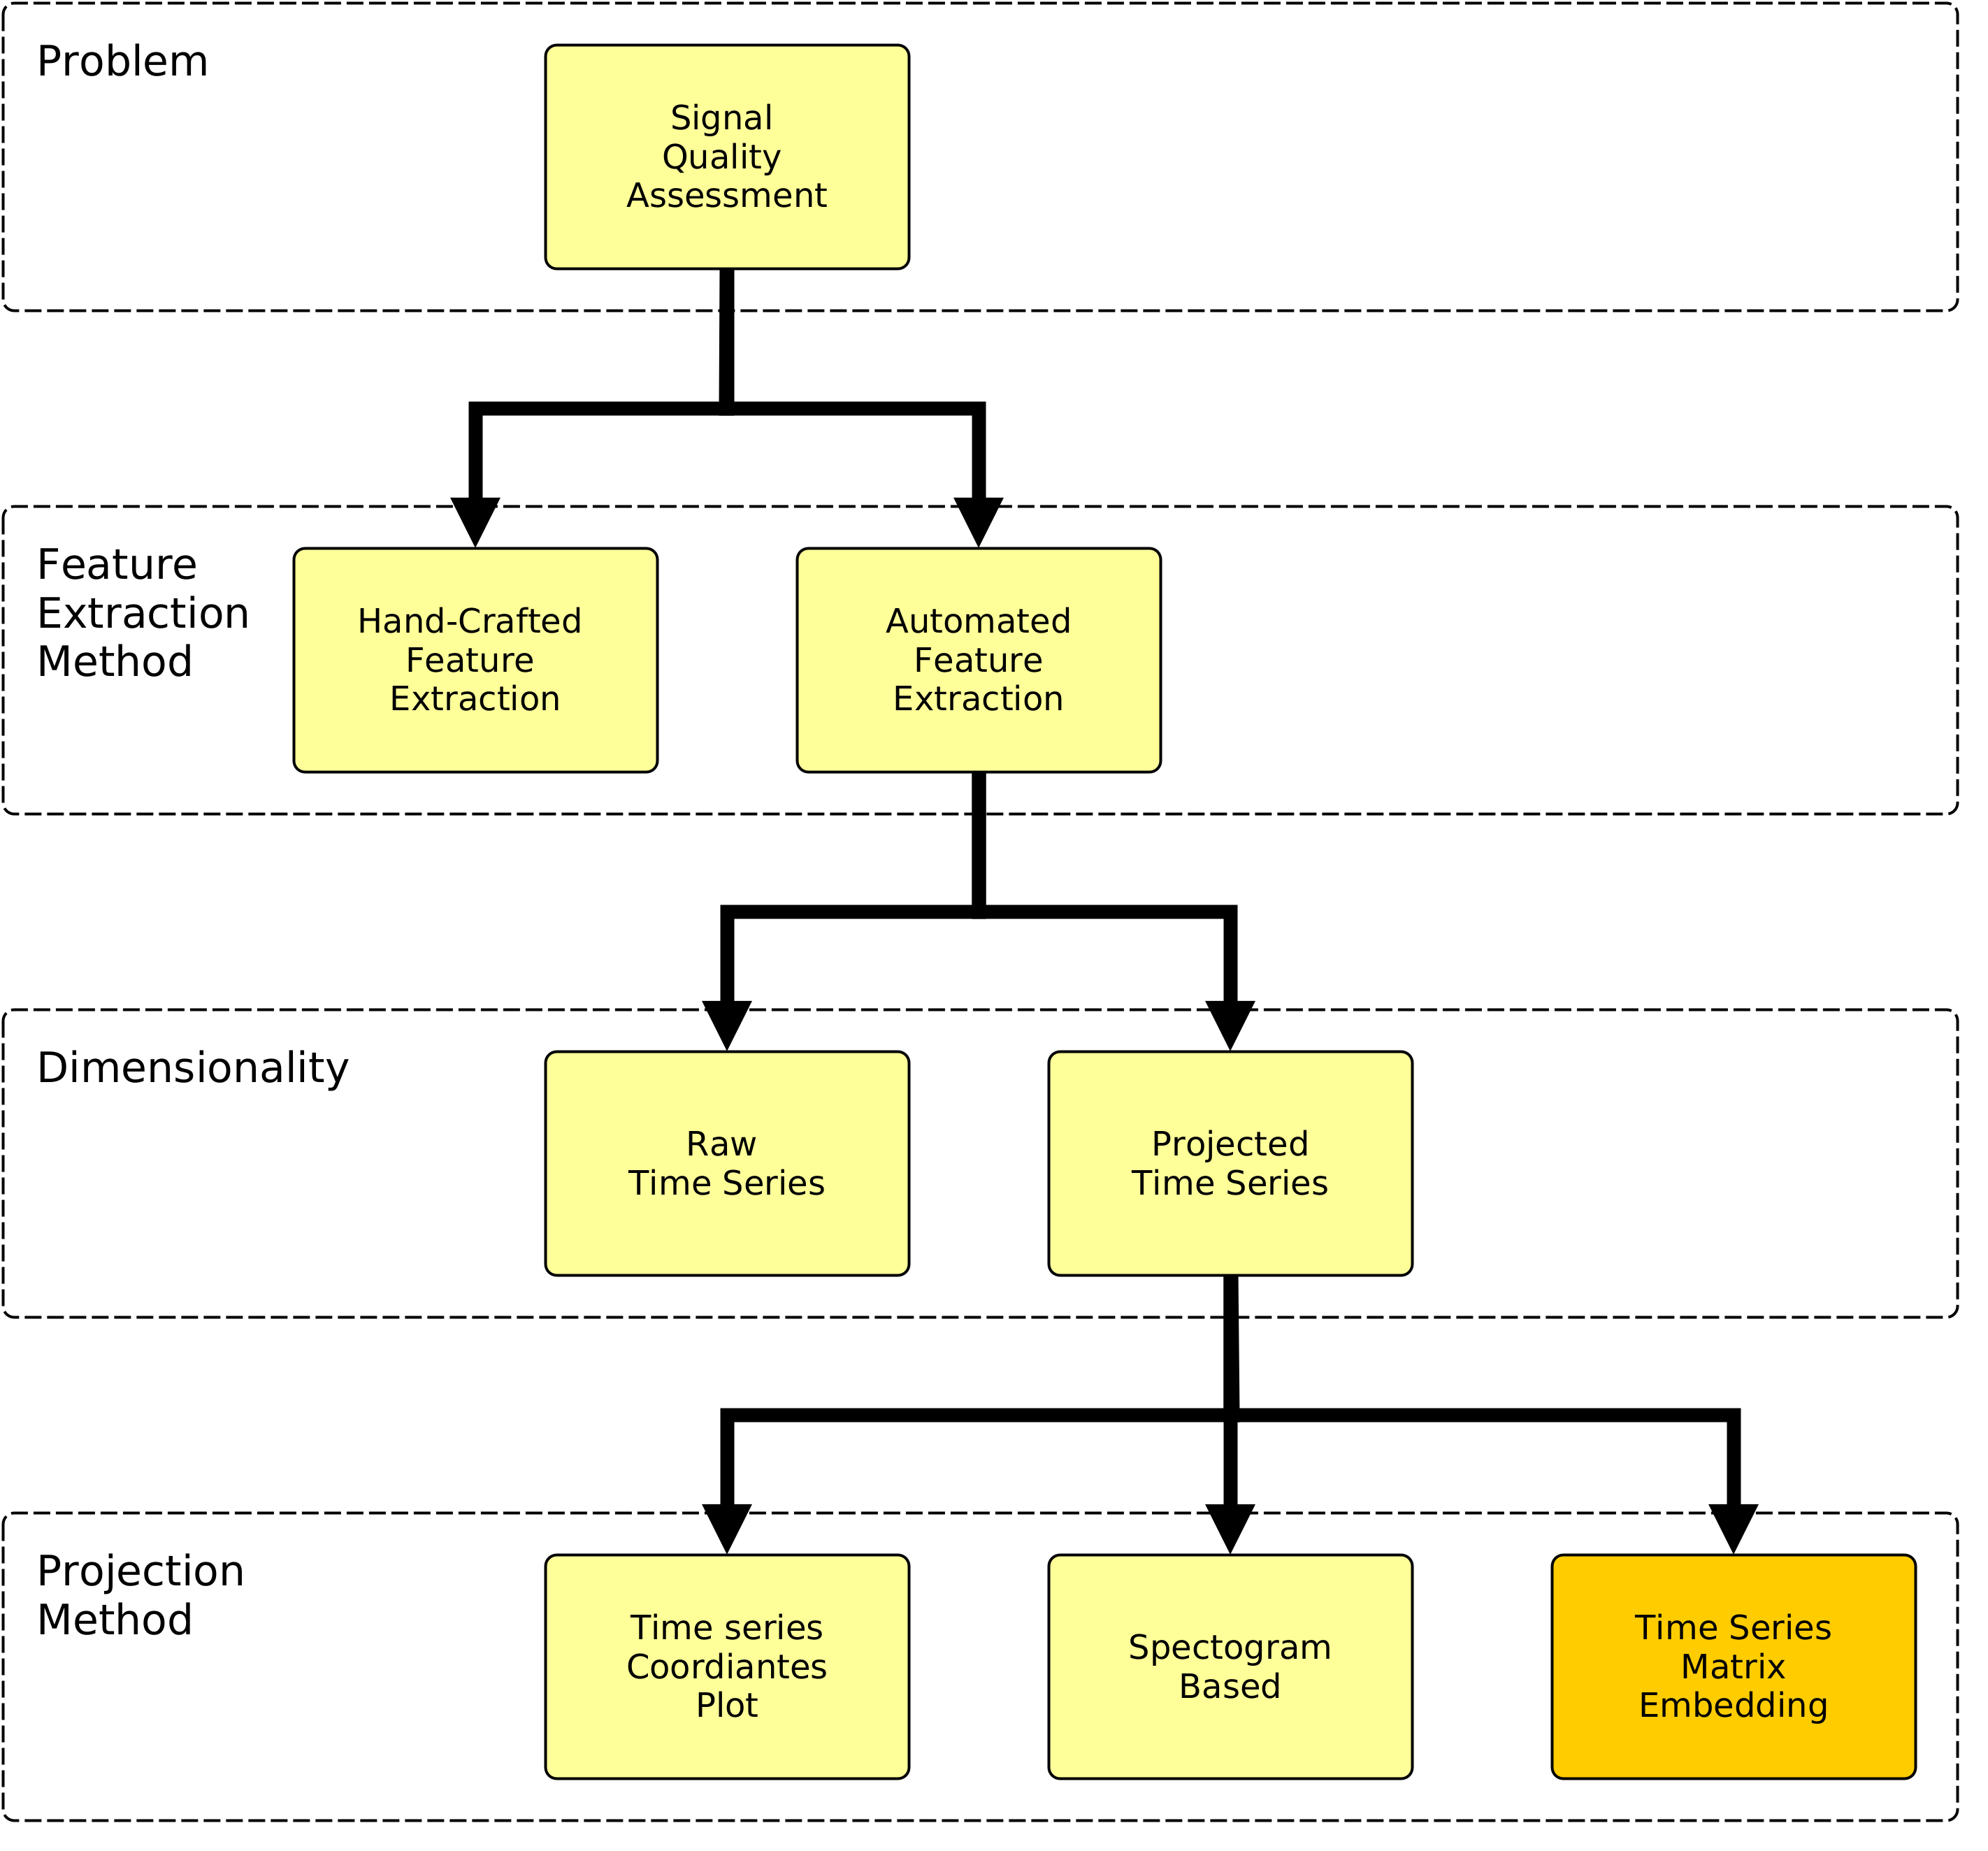
\includegraphics[width=\SubjectTreeSize]{img/SubjectTree.png}
	\caption{Visual schema of the \acrlong{SQA} literature state. It focuses in my work location, which I highlighted using the orange color.}
	\label{fig:SubjectTree}
\end{figure}


\section{The Problem}

% Usar outro exemplo para a tarefa de classificação.

In this section, I further specify the problem definition, according to the literature. This definition is not mathematically defined in the same manner for all researchers, since various delimitations could be proposed depending on the experiment method that they applied. But we can see that the literature treats the \acrshort{SQA} both as a regression and as a classification task. The regression perspective sees the \acrshort{SQA} as a tool for improving the estimation of continuous variables such as the \acrlong{HR}. For example, \citeauthor{review-1} proposes the use of a Naive Bayes classifier, that recieve metrics extracted from the signal, to provide the quality level to an Kalman filter which assesses the quality of the signal by fusing multiple observations \cite{review-1}. This improved the quality of the estimations \cite{review-1}. On the other hand, the classification point of view sees the \acrshort{SQA} as a isolated task of measuring the signal quality. A case of this is when \citeauthor{review-2} compared the input to a template signal by using the Dynamic Time Warping to measure a quality index that feeds a \acrshort{MLP}. In the end, this gives the quality class of the signal: ``good'' or ``bad'' \cite{review-2}. Despite that distinction, it is common to those two type of task that most works provide a \acrfull{SQI} to measure the quality of the signal, which we can also see in the researches that I mentioned in this paragraph.  

\section{The Feature Extraction Method}

As we saw, the \acrshort{SQI} is a common concept among the works. This index is a product of one or more features extracted from the input signal, which researchers achieved by a variety of methods. We can summarize those methods into two groups, as the Figure \ref{fig:SubjectTree} presents: one in which works extract hand-crafted features and another in which they use automated feature extraction, usually by employing deep learning algorithms. The oldest works, according to my knowledge, primally inserts into the hand-crafted features category. For instance, the oldest work that I found, made by \citeauthor{review-2}, designed a feature that measures the signal similarity to a template of a ideal signal by using the Dynamic Time Warping techinique \cite{review-2}. Then, \citeauthor{review-2} added this feature to other three and, finally, feeded them to a \acrshort{MLP}, which gives the \acrshort{SQI} of the signal \cite{review-2}. Since I will detail later the automated feature extraction, I will now focus on the oposite group.



\section{The Dimensionality}

\section{The Projection Method}

\section{This work contribution}
